\section{Computational Results}\label{sec:compResults}
\begin{equation} \label{eq:conslaw}
   \frac{\partial}{\partial t} \mathbf{u} + \nabla \cdot \mathbf{F} = 0
\end{equation}
\subsection{Linear convergence study}
We solve \eqref{eq:conslaw} with the flux $\mathbf{F}(u) = [-2\pi y u, 2\pi x u]$ and initial condition
$$
u_0(x,y) = w(\theta - \pi/2)
$$
where
$$
w(\theta) = \frac{1}{2}\left( \text{erf}\left( \frac{\pi/6 - \theta}{\sqrt{4/100}} \right) + \text{erf}\left( \frac{\pi/6 + \theta}{\sqrt{4/100}} \right)\right)
$$
until the final time $T = 1$ on the domain enclosed by two concentric discs of radii $R_1 = 0.751$ and $R_2 = 1.251$.  Figure \ref{fig:rotatinghillgrid} shows the computational domain embedded on a $50 \times 50$ grid.  The exact solution is the initial condition rotated about the point $(1.5,1.5)$, where $T=1$ corresponds to one solid body rotation.  The errors measured in the $L_1$ and $L_\infty$ norms are provided in Tables \ref{tab:ex1_L1} and \ref{tab:ex1_Linf}.
Figure
\ref{fig:rotatinghillexactiso} shows isolines of solution at the initial and final time.  The exact solution is applied as the boundary condition.

\begin{figure}
\subfloat[$50\times50$ grid and annulus domain.]{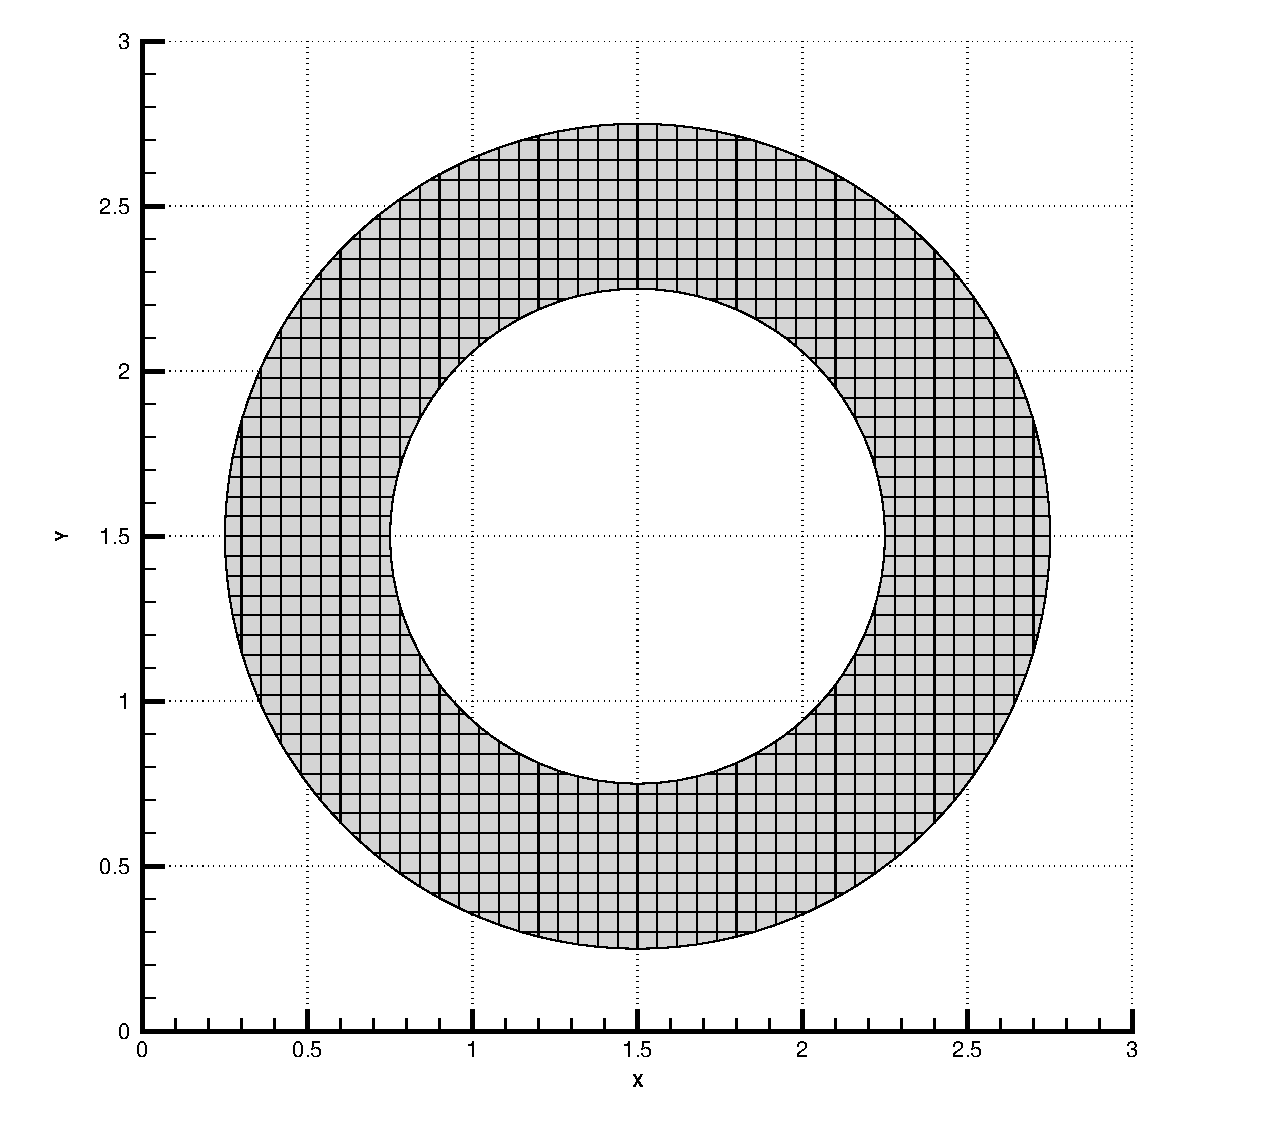
\includegraphics[width = 0.5\linewidth]{figs/rotatinghill_grid.eps} \label{fig:rotatinghillgrid}} 
\quad
\subfloat[Isolines of exact solution at the initial and final time.]{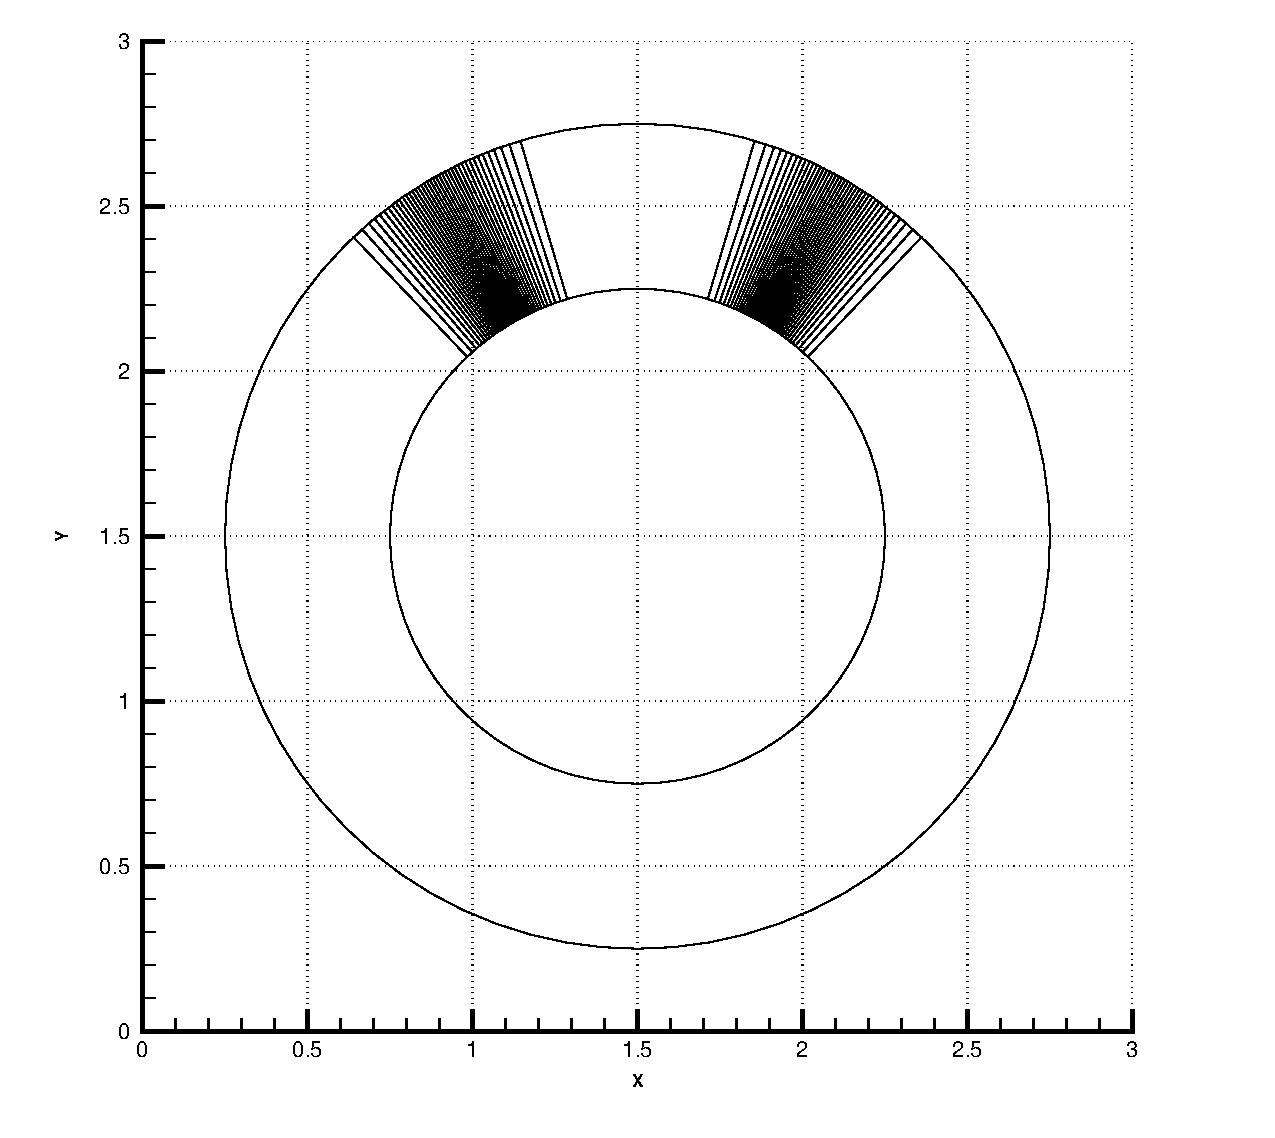
\includegraphics[width = 0.5\linewidth]{figs/rotatinghill_solution.eps}\label{fig:rotatinghillexactiso}}
\end{figure}
    % \caption{}\label{tab:ex1_L1}
\begin{table}
\centering
\subfloat[$L_1$ errors. \label{tab:ex1_L1}]{
    \begin{tabular}{|c|c|c|c|c|}
        \hline
         $N_x \times N_y$ & $p = 0$ & $p=1$& $p=2$ & $p=3$ \\
         \hline
         50 & 2.3937e-1(-) &  5.6588e-2  (-)& 4.1690e-2  (-)&   2.0694e-2 (-)\\
         \hline
         100 &  1.5521e-1 (0.62) &  2.0125e-2  (1.49)& 7.8165e-3 (2.41)& 1.6813e-3 (3.62)\\
         \hline
         200 &  9.4138e-2 (0.72) & 5.5222e-3 (1.86)&  9.98411e-4 (2.96)& 8.8527e-5 (4.24)\\
        %  \hline
        %  400 &  () &  ()&  ()&  ()\\
         \hline
    \end{tabular}
    }
\quad
\subfloat[$L_\infty$ errors. \label{tab:ex1_Linf}]{
    \begin{tabular}{|c|c|c|c|c|}
        \hline
         $N_x \times N_y$ & $p = 0$ & $p=1$& $p=2$ & $p=3$ \\
         \hline
         50 & 3.0385e-1 (-) &  1.6856e-1 (-)& 1.1809e-1 (-)&  7.0682e-2 (-)\\
         \hline
         100 & 2.3332e-1 (0.38) & 8.5487e-2 (1.04)& 5.1249e-2 (1.20)& 1.6657e-2 (2.08)\\
         \hline
         200 &  1.7698e-1 (0.39) & 3.4940e-2 (1.29)& 1.4500e-2 (1.82)&  1.9507e-3 (3.09)\\
        %  \hline
        %  400 &   () &  ()&  ()&  ()\\
         \hline
    \end{tabular}
    }

\caption{Errors for the linear convergence study.}
\end{table}

\subsection{Overlapping neighborhoods}
The purpose of this example is to demonstrate that our algorithm can handle overlapping neighborhoods. Using the streamfunction
$$
\phi = R - 0.25\sin(10\theta),
$$
with $R = \sqrt{(x-1.5)^2+(y-1.5)^2}$ and $\theta = \arctan((y-1.5)/(x-1.5))$, we define a linear flux based on the resulting divergence free velocity field, i.e.,  $\mathbf{F}(u) = [\phi_y u, -\phi_xu]$.  The characteristics of \eqref{eq:conslaw} lie on the isolines of the streamfunction.

A steady state solution to \eqref{eq:conslaw} with the above flux is given by the streamline function.  Therefore, we start with the initial condition given by the streamline function $\phi$, and compute the solution until the final time $T = 10$ on a $100 \times 100$ grid.  Additionally, we set the flux normal the domain boundary $\mathbf{F}\cdot \mathbf{n} = 0$.  This is to ensure that information does not leave the domain and should solution growth occur, this will more easily be noticed.



\begin{table}[h]
    \centering
    \subfloat[$L_1$ errors.]{
    \begin{tabular}{|c|c|c|c|}
    \hline
        $p = 0$ & $p =1$ & $p = 2$ & $p =3$  \\
        \hline
        3.8585e-1 & 3.6118e-2 & 8.29907e-3 & 4.3116e-3\\
        \hline
    \end{tabular} \label{tab:errorsteadystatel1}
    }
    \quad
\subfloat[$L_\infty$ errors.]{
    \begin{tabular}{|c|c|c|c|}
    \hline
        $p = 0$ & $p =1$ & $p = 2$ & $p =3$  \\
        \hline
        2.9470e-1 & 9.5323e-2 & 2.4851e-2 &  5.4720e-3 \\
        \hline
    \end{tabular}
    \label{tab:errorsteadystatelinfty}
    }
    
\caption{Errors for overlapping neighborhoods study.} \label{tab:overlappingerrors}
\end{table}

\begin{figure}[h]
%\subfloat[Isolines of exact solution at the initial and final time.]{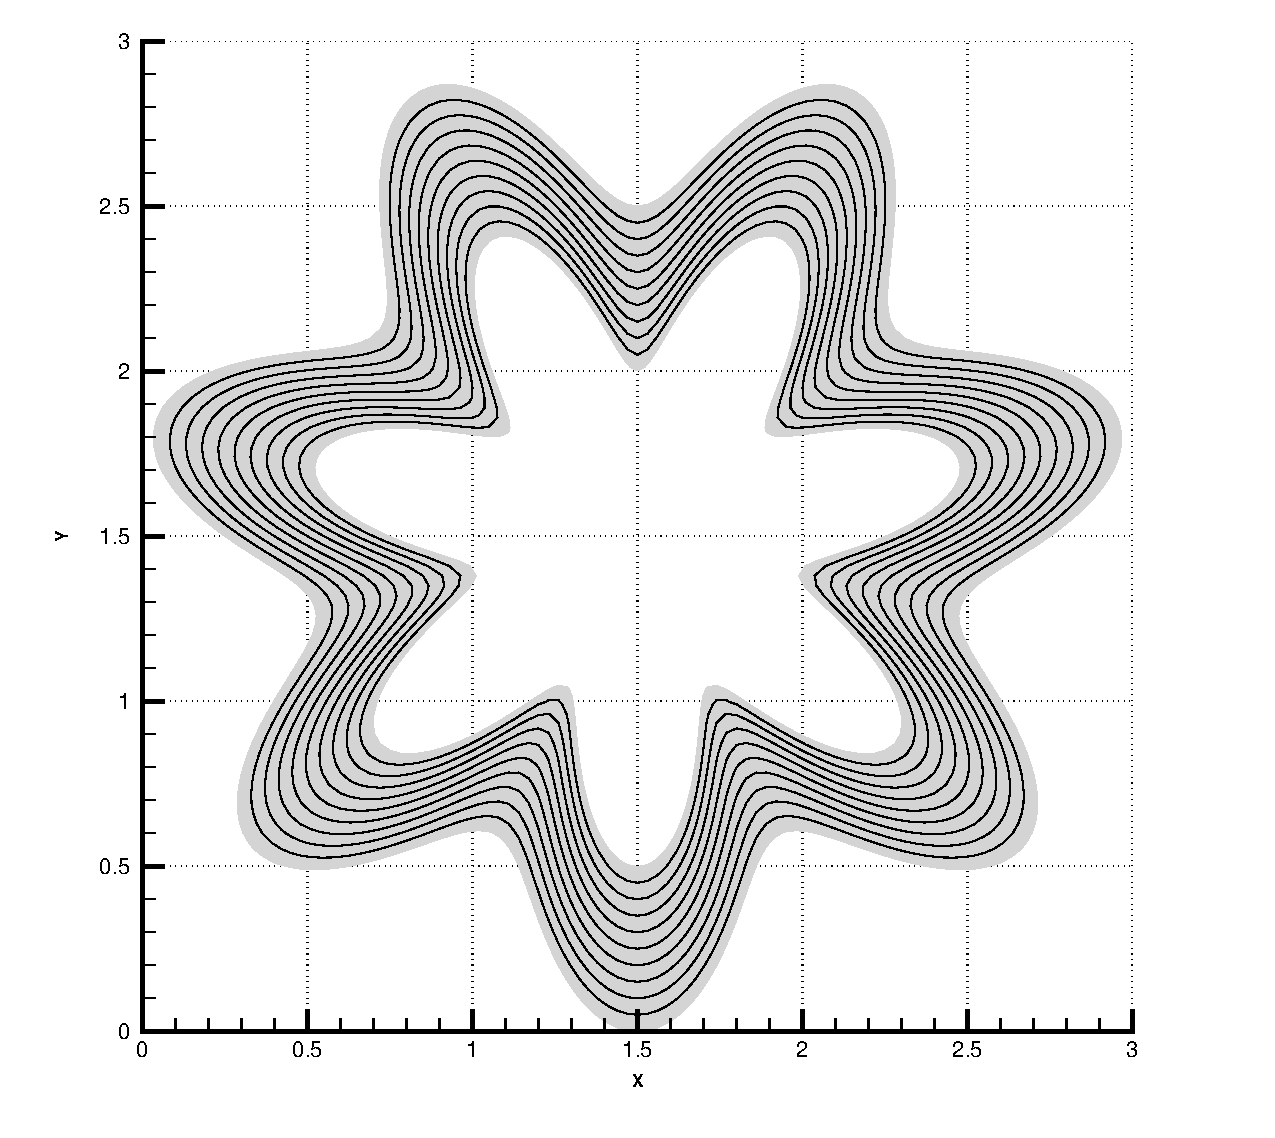
\includegraphics[width = 0.5\linewidth]{figs/waveyiso.eps} \label{fig:waveyisolines}} 
%\subfloat[Isolines of exact solution at the initial and final time.]{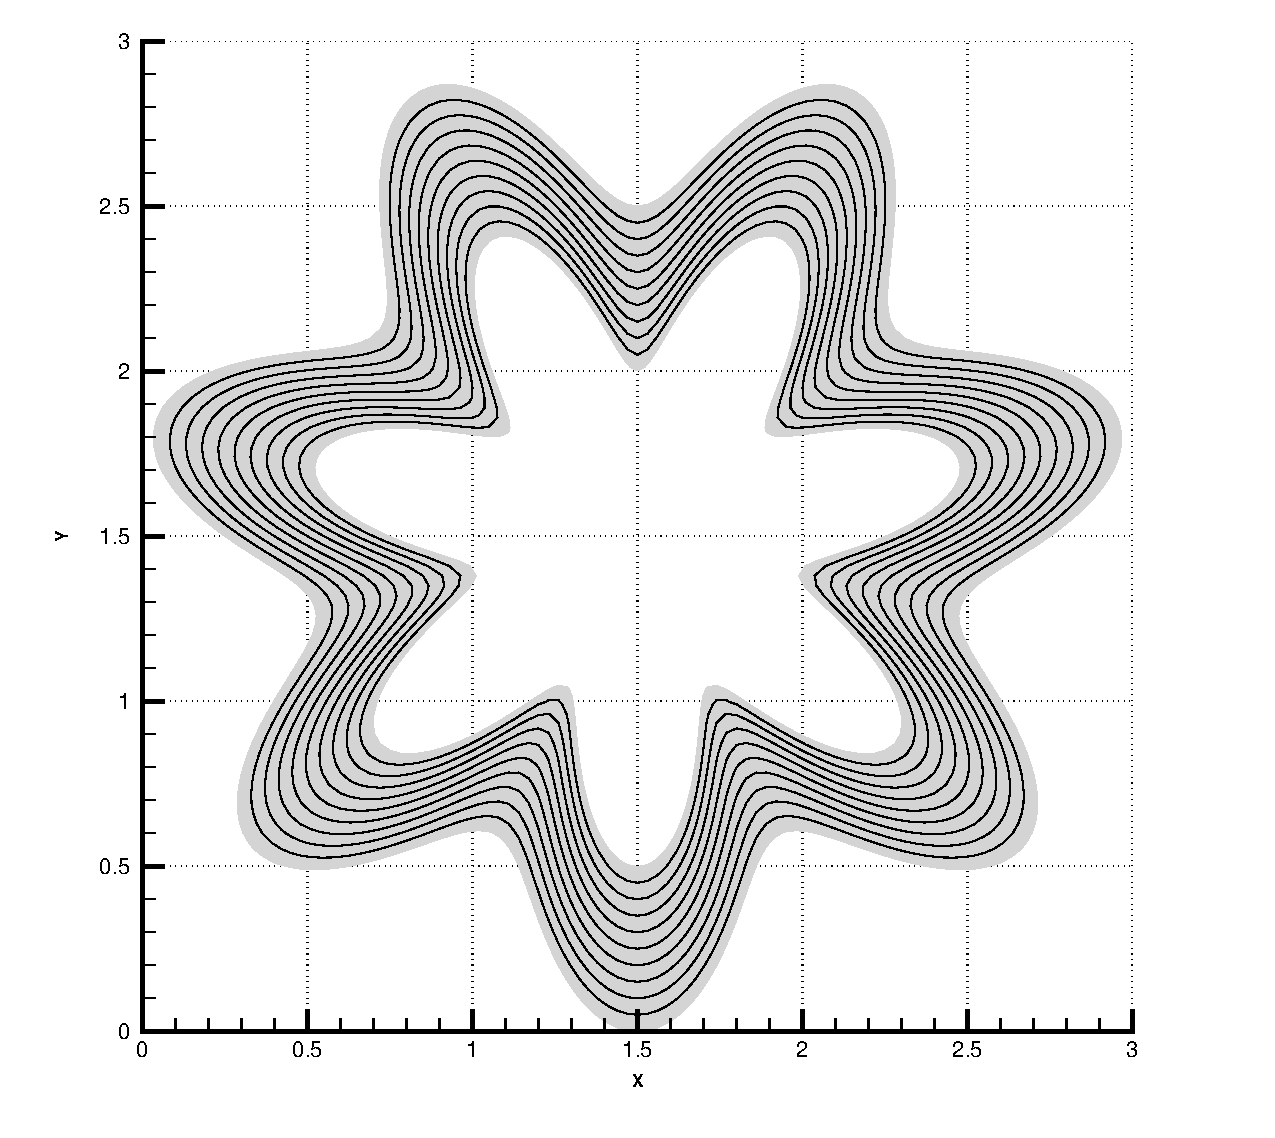
\includegraphics[width = 0.5\linewidth]{figs/waveyiso.eps} \label{fig:waveyisolines}} 
%\quad
\subfloat[Number of overlapping merging neighborhoods: one (blue), two (green), three (red).]{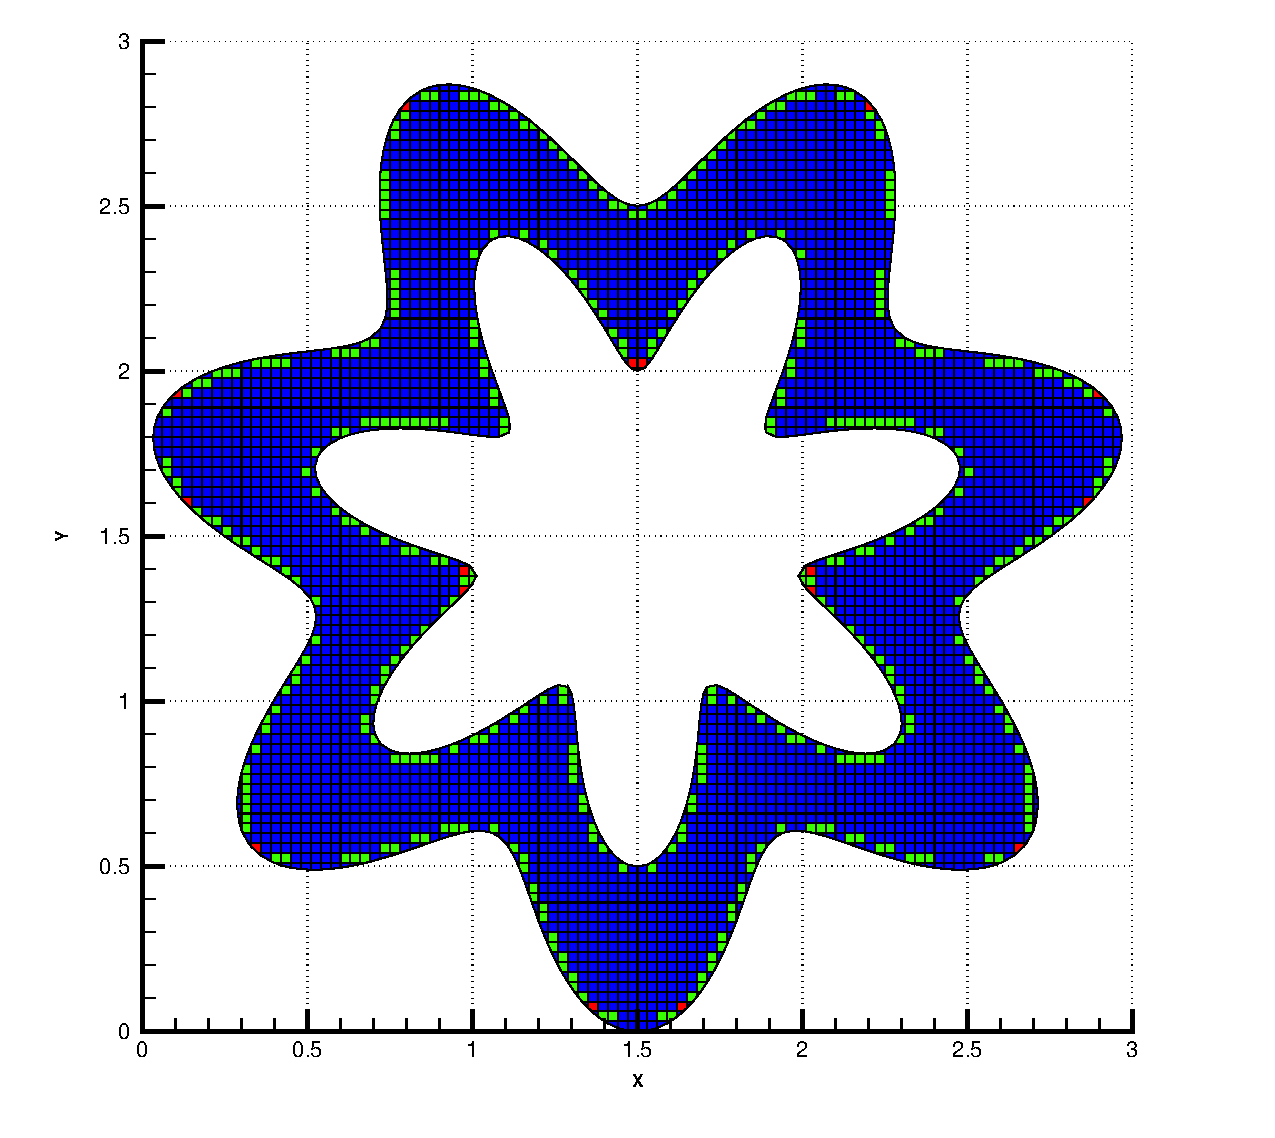
\includegraphics[width = 0.5\linewidth]{figs/waveynumhoods.eps}\label{fig:waveynumhoods}}
% 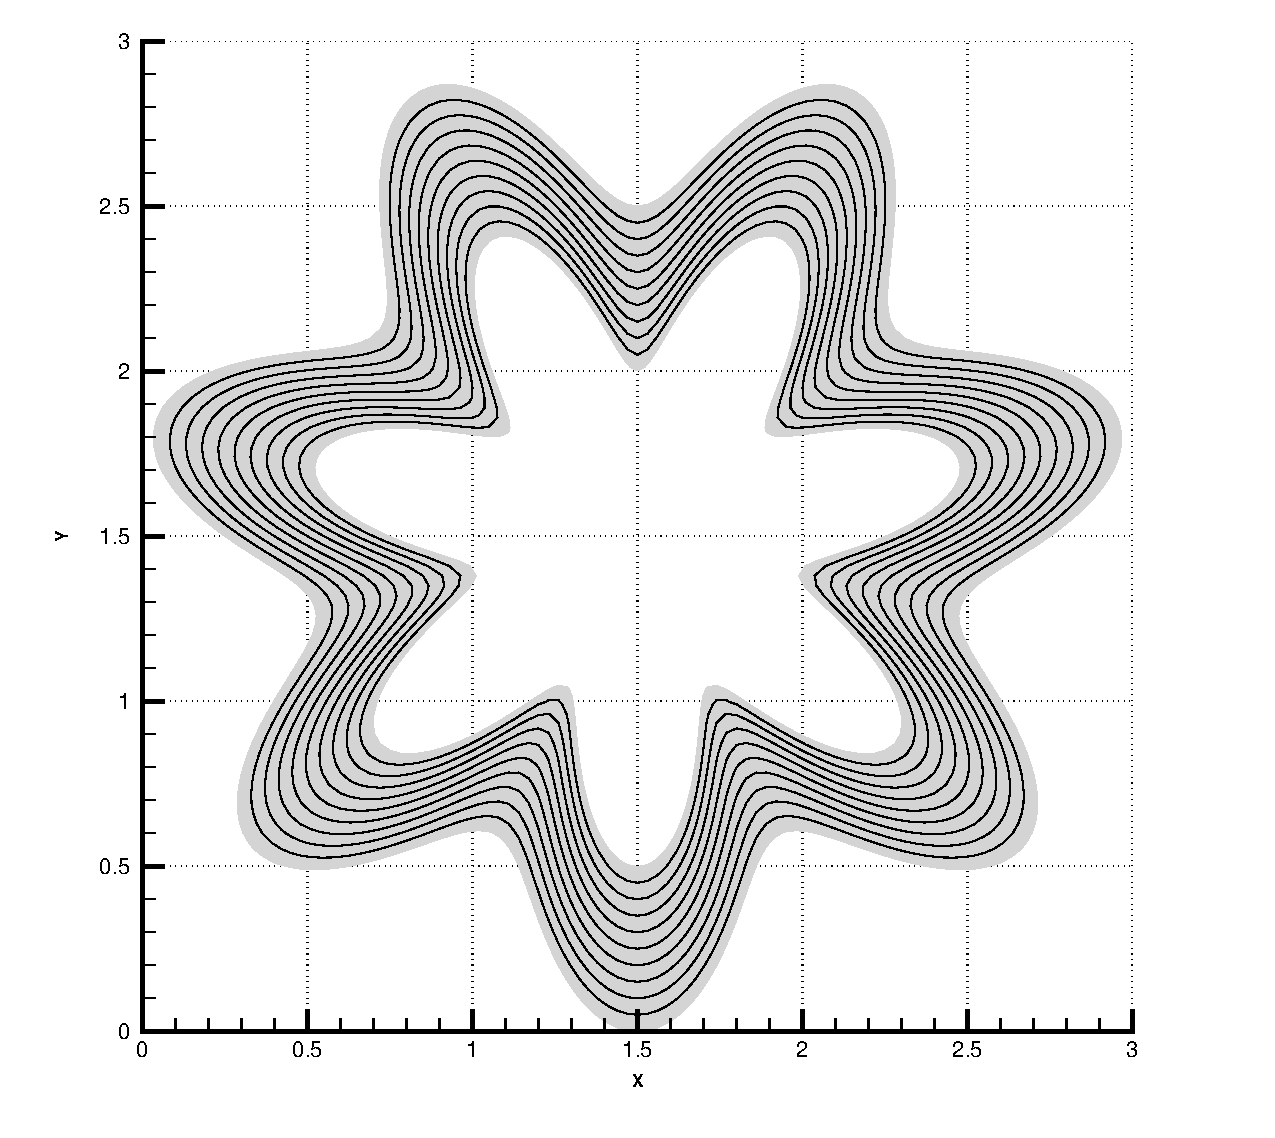
\includegraphics[width = 0.5\linewidth]{figs/waveyiso.eps} 
\subfloat[Isolines of exact solution at the initial and final time.]{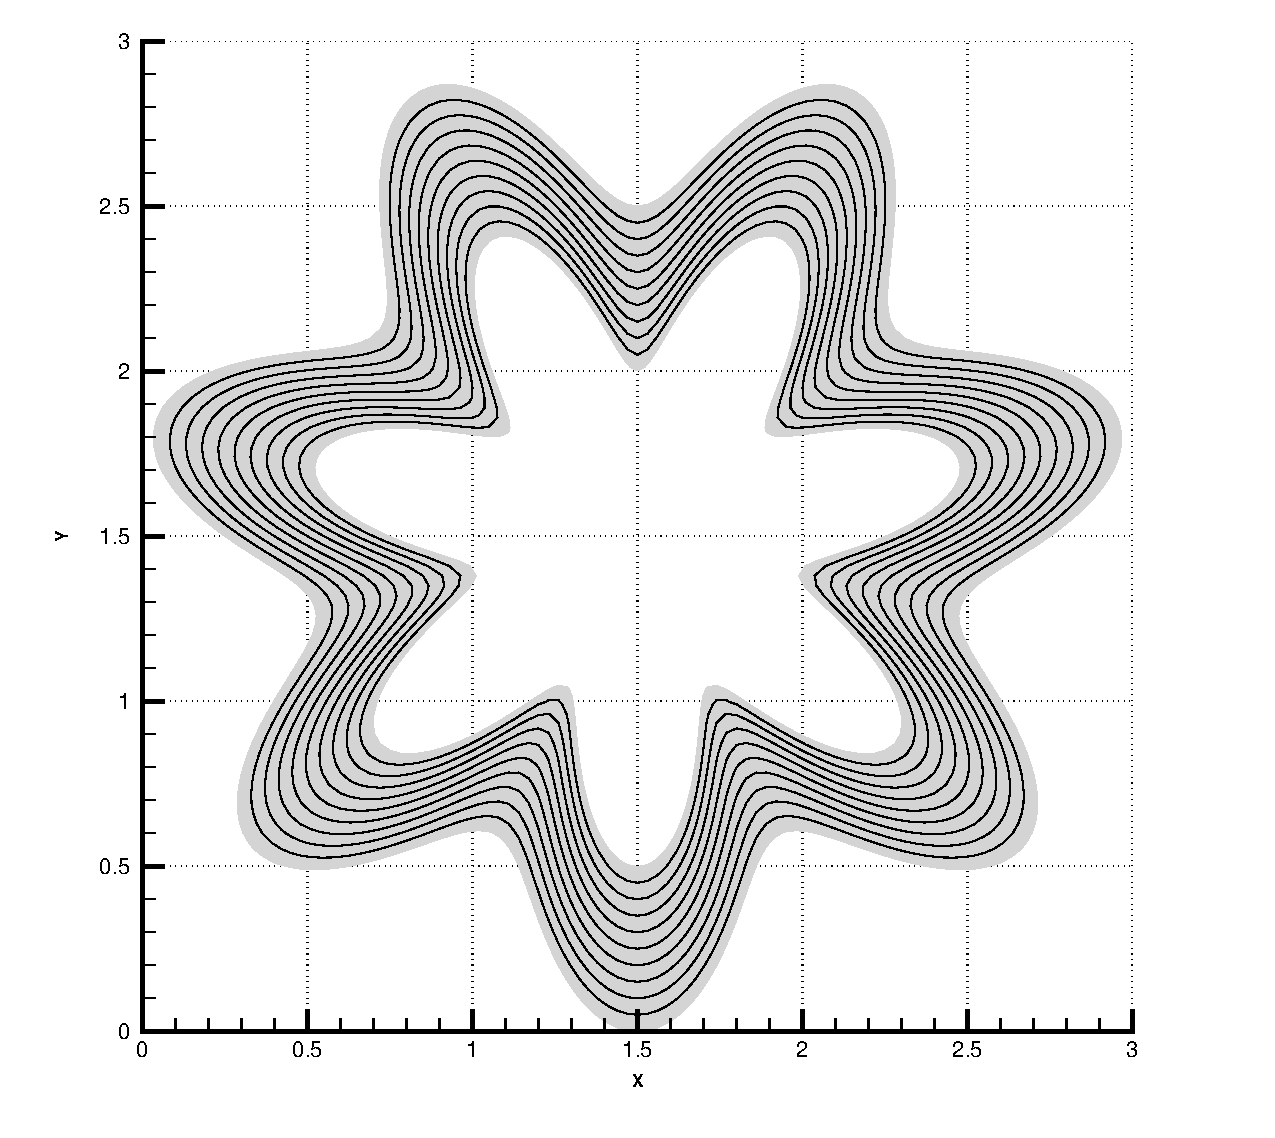
\includegraphics[width = 0.5\linewidth]{figs/waveyiso.eps} \label{fig:waveyisolines}} 
\caption{Isolines of exact solution at the initial and final time for the wavy domain with overlapping neighborhoods.} 
% \label{fig:overlappingneighborhoods}
% \label{fig:waveyisolines}} 
\end{figure}

In Figure \ref{fig:waveyisolines}, we show the isolines of the exact solution at the initial and final times.  Additionally, Figure \ref{fig:waveynumhoods} shows the number of overlapping neighborhoods on each cell.  In this example, we have at most three overlapping neighborhoods.  They are concentrated where the boundary has high curvature.   We do not observe growth in the numerical solution as indicated by $L_1$ and $L_\infty$ errors of the solution at the final time listed in Table \ref{tab:overlappingerrors}.  Although this experiment does not prove stability of our numerical scheme, not observing unbounded growth in the numerical solution is a necessary condition.


\subsection{Nonlinear convergence study}
We solve the supersonic vortex problem which describes supersonic flow 
through a tube.  This problem has often been used in accuracy studies
because it has an exact solution \cite{aftosmis:acc}, given by 
$$
\begin{pmatrix}
\rho\\
u \\
v \\
p
\end{pmatrix} = \begin{pmatrix}
[1 + 1.0125(1-r^{-2})]^{2.5}\\
2.25r^{-1}\sin(\theta)\\
-2.25r^{-1}\cos(\theta)\\
\frac{1}{\gamma}\rho^{\gamma}
\end{pmatrix},
$$
where $r = \sqrt{x^2+y^2}$.  The exact solution is applied to the inflow 
and outflow, i.e., the horizontal and vertical boundaries.  
High-order reflecting boundary conditions are used on the curved
boundaries as in \cite{}, even though  the  actual embedded boudnary is
represented by a linear segment in each cut cell.  

The simulation is run until a steady state is reached, defined by 
$$
\max_{i,j}|U^{n+1}_{i,j}-U^{n}_{i,j}| < 10^{-10}.
$$
The $L_1$ and $L_\infty$ errors are given in Table \ref{tab:ex2_L1} and \ref{tab:ex2_Linf}.

% \begin{table}
% \centering
% \subfloat[$L_1$ errors. \label{tab:ex2_L1}]{
%     \begin{tabular}{|c|c|c|c|c|}
%         \hline
%          $N_x \times N_y$ & $p = 0$ & $p=1$& $p=2$ & $p=3$ \\
%          \hline
%          50 & 9.4739e-2 (-) & 5.0410e-3  (-)& 1.1052e-3 (-)& 5.0620e-4 (-)\\
%          \hline
%          100 & 4.8604e-2  (0.96) & 1.4182e-3 (1.82)& 1.7253e-4 (2.67) & 3.41009e-5 (3.89)\\
%          \hline
%          200 &  2.5369e-2  (0.93) &   3.3332e-4  ()&  ()& ()\\
%         %  \hline
%         %  400 &  () &  ()&  ()&  ()\\
%          \hline
%     \end{tabular}
%     }
% \quad
% \subfloat[$L_\infty$ errors. \label{tab:ex2_Linf}]{
%     \begin{tabular}{|c|c|c|c|c|}
%         \hline
%          $N_x \times N_y$ & $p = 0$ & $p=1$& $p=2$ & $p=3$ \\
%          \hline
%          50 &  5.4474e-1 (-) &  2.3337e-2 (-)& 9.5250e-3 (-)& 2.1902e-3 (-)\\
%          \hline
%          100 &  3.0634e-1 (0.83) &  8.5984e-3  (1.44)& 3.2008e-3 (1.44)& 2.8438e-4 (2.94)\\
%          \hline
%          200 &  1.6236e-1  (0.91) &  3.7170e-3  ()&  ()& ()\\
%         %  \hline
%         %  400 &   () &  ()&  ()&  ()\\
%          \hline
%     \end{tabular}
%     }

% \caption{Errors for the nonlinear convergence study.}
% \end{table}

\begin{table}
\centering
\subfloat[$L_1$ errors. \label{tab:ex2_L1}]{
    \begin{tabular}{|c|c|c|c|c|}
        \hline
         $N_x \times N_y$ & $p = 0$ & $p=1$& $p=2$ & $p=3$ \\
         \hline
         50 &9.5684e-2 (-) & 2.5288e-3 (-)& 1.0461e-3 (-)& 4.5228e-4 (-)\\
         \hline
         100 & 4.8806e-2 (0.97) & 8.4046e-4  (1.58)& 1.6831e-4 (2.68) & 3.2118e-5 (3.81)\\
         \hline
         200 & 2.5311e-2 (0.94) & 1.9726e-4 (2.09)& 2.3377e-5 (2.84) & 1.9907e-6 (4.01)\\
        %  \hline
        %  400 &  () &  ()&  ()&  ()\\
         \hline
    \end{tabular}
    }
\quad
\vspace*{.2in}

\subfloat[$L_\infty$ errors. \label{tab:ex2_Linf}]{
    \begin{tabular}{|c|c|c|c|c|}
        \hline
         $N_x \times N_y$ & $p = 0$ & $p=1$& $p=2$ & $p=3$ \\
         \hline
         50 & 5.4756e-1 (-) & 1.8694e-2 (-)& 7.2911e-3 (-)& 1.9752e-3 (-)\\
         \hline
         100 & 3.0527e-1 (0.84) & 6.9103e-3 (1.43)& 1.5457e-3 (2.23) & 1.5927e-4 (3.63)\\
         \hline
         200 & 1.6319e-1  (0.90) &  2.4883e-3 (1.47)& 4.2102e-4 (1.87) & 1.5372e-5 (3.37)\\
        %  \hline
        %  400 &   () &  ()&  ()&  ()\\
         \hline
    \end{tabular}
    }

\caption{Errors for the nonlinear convergence study.}
\end{table}

NEED TO COMPARE TO OTHER ANSWERS, MAYBE INCLUDE  ERROR PLOT

\subsection{Double Mach Reflection problem}
